% ---------------------------------------------------------------- 25c Math: label -> channels -> label
\begin{frame}{One chain --- from the label to the channels, and back}
  \setlength{\abovedisplayskip}{5pt}
  \setlength{\belowdisplayskip}{5pt}
  \small
  Take one pixel and follow its parameters through the physics. Every symbol
  used in this discussion is introduced on its own line:

  \[
  \begin{aligned}
    & p(z) \;=\; \textstyle\sum_k a_k\,\mathcal N(z;\mu_k,\sigma_k)
        && \text{\scriptsize\color{soft} the label: scales $a_k$, elevations $\mu_k$, widths $\sigma_k$, along elevation $z$}\\[4pt]
    \Longrightarrow\;\; & \mathrm E[\gamma(z)\,\gamma^*(z')] \;=\; p(z)\,\delta(z{-}z')
        && \text{\scriptsize\color{soft} $\gamma$: the pixel's speckled reflectivity --- random, with power profile $p$}\\[4pt]
    \Longrightarrow\;\; & g_n \;=\; \textstyle\int \gamma(z)\,e^{\,jk_nz}\,dz \;=\; A_n\,e^{\,j\theta_n}
        && \text{\scriptsize\color{soft} pass $n$: one Fourier coefficient, at frequency $k_n \propto$ baseline $b_{\perp,n}$}\\[4pt]
    \Longrightarrow\;\; & \underbrace{A_0,\dots,A_4}_{\text{5 amplitudes}}\,, \quad \underbrace{\varphi_n = \theta_0-\theta_n}_{\text{4 IFG phases}}
        && \text{\scriptsize\color{soft} the nine input channels: $A_n=|g_n|$,\; $\theta_n=\arg g_n$}\\[4pt]
    \Longrightarrow\;\; & \hat R_{mn} \;=\; \big\langle A_mA_n\,e^{\,j(\varphi_n-\varphi_m)} \big\rangle_{B(x)} \;\approx\; P\,\rho(k_m{-}k_n)
        && \text{\scriptsize\color{soft} covariance over the window $B(x)$: $\theta_0$ cancels; $P{=}\int p$,\; $\rho{=}\mathrm{FT}[p/P]$}\\[4pt]
    \Longrightarrow\;\; & \hleq{\mathrm{Capon}(\hat R) \;\to\; \hat p \;\to\; \text{fit} \;\to\; a_k,\ \mu_k,\ \sigma_k}
        && \text{\scriptsize\color{soft} the GT pipeline --- the same parameters return}
  \end{aligned}
  \]

  \smallskip
  The loop closes: the nine channels contain everything the label was built
  from. An ablation can only \emph{delete} information --- the next two chains
  show which parameter each half can never see.
\end{frame}

% ---------------------------------------------------------------- 25d Math: the two invariances
\begin{frame}{Two exact invariances}
  \setlength{\abovedisplayskip}{4pt}
  \setlength{\belowdisplayskip}{4pt}
  \begin{columns}[c]
    \begin{column}{0.49\textwidth}
      \small
      \begin{itemize}
        \item \textbf{Amplitudes are shift-blind.}
              Move the whole profile up by $\Delta$:
      \end{itemize}
      \[
      \begin{aligned}
        & p(z) \;\to\; p(z-\Delta)\\[3pt]
        \Longrightarrow\;\; & \gamma(z) \;\to\; \gamma(z-\Delta)\\[3pt]
        \Longrightarrow\;\; & g_n \;\to\; e^{\,jk_n\Delta}\,g_n\\[3pt]
        \Longrightarrow\;\; & \hleq{A_n = |e^{\,jk_n\Delta}|\,|g_n| \;\;\text{unchanged}}
      \end{aligned}
      \]
      Position never reaches an amplitude --- 29 of them are as blind as 5.
      What they still carry:
      \[
      \begin{aligned}
        & \hleq{\mathrm E[A_n^2] \;=\; P \;\;\Longrightarrow\;\; \text{the scale } a}\\[3pt]
        & \hleq{\mathrm{cov}(A_m^2,A_n^2) \;=\; P^2\,|\rho(k_m{-}k_n)|^2 \;\;\Longrightarrow\;\; \sigma,\ \Delta\mu}
      \end{aligned}
      \]
      Scale and shape ($\sigma$, separation $\Delta\mu$) survive; the position
      $\mu$ is gone.
    \end{column}
    \begin{column}{0.49\textwidth}
      \small
      \begin{itemize}
        \item \textbf{Phases are scale-blind.}
              Scale the whole profile by $c>0$:
      \end{itemize}
      \[
      \begin{aligned}
        & p(z) \;\to\; c\,p(z)\\[3pt]
        \Longrightarrow\;\; & \gamma(z) \;\to\; \sqrt{c}\,\gamma(z)\\[3pt]
        \Longrightarrow\;\; & g_n \;\to\; \sqrt{c}\,g_n\\[3pt]
        \Longrightarrow\;\; & \hleq{\varphi_n = \theta_0-\theta_n \;\;\text{unchanged}}
      \end{aligned}
      \]
      Scale never reaches a phase. What they still carry --- the shape $\rho$
      at frequency $\kappa$, for one scatterer at $\mu$, width $\sigma$:
      \[
      \begin{aligned}
        & \rho(\kappa) \;=\; e^{\,j\kappa\mu}\,e^{-\kappa^2\sigma^2/2}\\[3pt]
        \Longrightarrow\;\; & \hleq{\arg\rho(k_n) = k_n\,\mu \;\;\Longrightarrow\;\; \text{a line of slope } \mu}\\[3pt]
        \Longrightarrow\;\; & \hleq{|\rho(k_n)| = e^{-k_n^2\sigma^2/2} \;\;\Longrightarrow\;\; \text{phase spread} \to \sigma}
      \end{aligned}
      \]
      Position is read directly; a second scatterer bends the line ---
      detection.
    \end{column}
  \end{columns}
\end{frame}

% ---------------------------------------------------------------- 25e Math: the partition and the two error costs
\begin{frame}{Putting the two invariances together}
  \setlength{\abovedisplayskip}{1pt}
  \setlength{\belowdisplayskip}{1pt}
  \begin{columns}[c]
    \begin{column}{0.49\textwidth}
      \small
      \begin{itemize}
        \item \textbf{The shift error.} One component
              $\mathcal N_\mu = \mathcal N(z;\mu,\sigma)$ of energy
              $E=\lVert\mathcal N_\mu\rVert^2$; the prediction lands $\delta$ away:
      \end{itemize}
      \[
      \begin{aligned}
        & \lVert \mathcal N_{\mu+\delta}-\mathcal N_{\mu}\rVert^2 \;=\; 2E \,-\, 2\,\langle \mathcal N_{\mu+\delta},\,\mathcal N_{\mu}\rangle\\[2pt]
        \Longrightarrow\;\; & \langle \mathcal N_{\mu+\delta},\,\mathcal N_{\mu}\rangle \;=\; E\,e^{-\delta^2/4\sigma^2}\\[2pt]
        \Longrightarrow\;\; & \lVert \mathcal N_{\mu+\delta}-\mathcal N_{\mu}\rVert^2 \;=\; 2E\,\big(1-e^{-\delta^2/4\sigma^2}\big)\\[2pt]
        \Longrightarrow\;\; & \hleq{\delta\ll\sigma:\ \approx E\,\delta^2/2\sigma^2, \qquad \delta\gg\sigma:\ \to 2E}
      \end{aligned}
      \]
      {\scriptsize\color{soft} $\langle f,g\rangle=\int\! fg$: the overlap;
      $\lVert f\rVert^2=\langle f,f\rangle$: the energy --- only the cross-term moves.\par}
      \smallskip
      \begin{itemize}
        \item \textbf{The scale error.} The same component, its brightness off
              by the relative error $\varepsilon$:
      \end{itemize}
      \[
      \begin{aligned}
        & \lVert (1{+}\varepsilon)\,\mathcal N_\mu-\mathcal N_{\mu}\rVert^2 \;=\; \lVert \varepsilon\,\mathcal N_\mu\rVert^2 \;=\; \varepsilon^2E\\[2pt]
        \Longrightarrow\;\; & \hleq{\varepsilon^2E = 2E \ \text{only at}\ \varepsilon=\sqrt2 \ \text{--- a 141\% error}}
      \end{aligned}
      \]
    \end{column}
    \begin{column}{0.49\textwidth}
      \small
      \begin{itemize}
        \item \textbf{Take the derivative of each error:}
      \end{itemize}
      \[
      \begin{aligned}
        & \tfrac{d}{d\delta}\,\lVert \mathcal N_{\mu+\delta}-\mathcal N_{\mu}\rVert^2 \;=\; \tfrac{E\,\delta}{\sigma^2}\;e^{-\delta^2/4\sigma^2} \;\xrightarrow{\;\delta\gg\sigma\;}\; 0\\[1pt]
        \Longrightarrow\;\; & \hleq{\text{the shift error flattens: } 2E \text{ is a true maximum}}\\[1pt]
        & \tfrac{d}{d\varepsilon}\,\lVert (1{+}\varepsilon)\,\mathcal N_\mu-\mathcal N_{\mu}\rVert^2 \;=\; 2\,\varepsilon E \;>\; 0 \ \text{ at every } \varepsilon\\[1pt]
        \Longrightarrow\;\; & \hleq{\text{the scale error never flattens}}
      \end{aligned}
      \]
      \smallskip
      \begin{columns}[T]
        \begin{column}{0.48\linewidth}
          \centering
          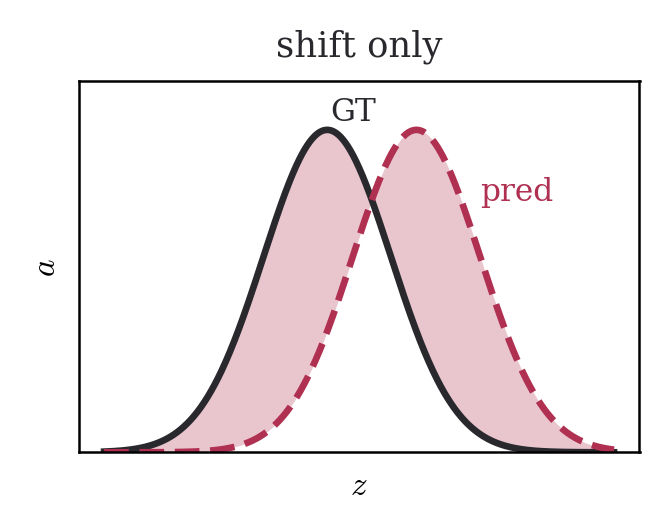
\includegraphics[width=\linewidth]{../figures/error_landscape/shift_only_profile.png}
        \end{column}
        \begin{column}{0.48\linewidth}
          \centering
          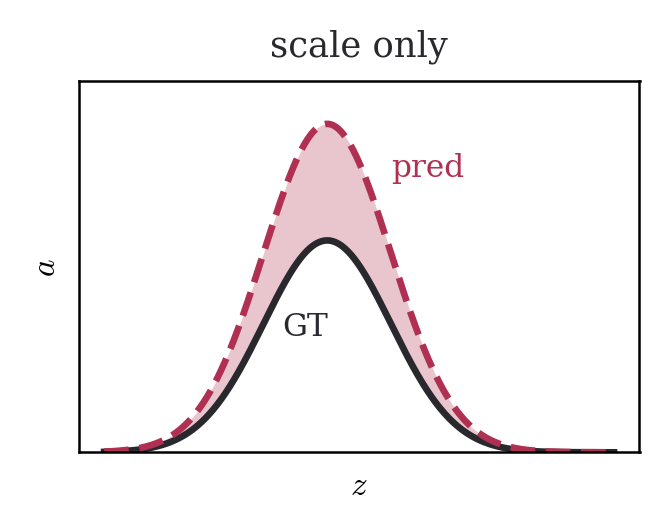
\includegraphics[width=\linewidth]{../figures/error_landscape/scale_only_profile.png}
        \end{column}
      \end{columns}
    \end{column}
  \end{columns}
\end{frame}

% ---------------------------------------------------------------- 25e-b Math: the joint error landscape
\begin{frame}{Shift and scale together --- the joint error}
  \setlength{\abovedisplayskip}{3pt}
  \setlength{\belowdisplayskip}{3pt}
  \begin{columns}[c]
    \begin{column}{0.52\textwidth}
      \small
      \begin{itemize}
        \item \textbf{Both mistakes at once} --- the prediction scaled by
              $1{+}\varepsilon$ \emph{and} misplaced by $\delta$:
      \end{itemize}
      \[
      \begin{aligned}
        & \lVert (1{+}\varepsilon)\,\mathcal N_{\mu+\delta}-\mathcal N_{\mu}\rVert^2\\[2pt]
        \Longrightarrow\;\; & \;=\; (1{+}\varepsilon)^2E + E - 2\,(1{+}\varepsilon)\,\langle\mathcal N_{\mu+\delta},\,\mathcal N_{\mu}\rangle\\[2pt]
        \Longrightarrow\;\; & \hleq{\;=\; E\,\big[(1{+}\varepsilon)^2 + 1 - 2\,(1{+}\varepsilon)\,e^{-\delta^2/4\sigma^2}\big]}\\[2pt]
        \Longrightarrow\;\; & \varepsilon{=}0:\ 2E\big(1-e^{-\delta^2/4\sigma^2}\big), \qquad \delta{=}0:\ \varepsilon^2E
      \end{aligned}
      \]

      \smallskip
      \begin{itemize}
        \item \textbf{Take the partial derivatives:}
      \end{itemize}
      \[
      \begin{aligned}
        & \tfrac{\partial}{\partial\delta}\,\lVert(1{+}\varepsilon)\,\mathcal N_{\mu+\delta}-\mathcal N_{\mu}\rVert^2 \;=\; (1{+}\varepsilon)\,\tfrac{E\,\delta}{\sigma^2}\,e^{-\delta^2/4\sigma^2}\\[2pt]
        & \tfrac{\partial}{\partial\varepsilon}\,\lVert(1{+}\varepsilon)\,\mathcal N_{\mu+\delta}-\mathcal N_{\mu}\rVert^2 \;=\; 2E\,\big(1{+}\varepsilon-e^{-\delta^2/4\sigma^2}\big)\\[2pt]
        \Longrightarrow\;\; & \tfrac{\partial}{\partial\delta} = 0 \ \text{ at } \ \delta \;=\; 0 \ \text{ (any } \varepsilon)\\[2pt]
        \Longrightarrow\;\; & \hleq{\tfrac{\partial}{\partial\varepsilon} = 0 \ \text{ at } \ 1{+}\varepsilon \;=\; e^{-\delta^2/4\sigma^2} \;<\; 1}
      \end{aligned}
      \]
    \end{column}
    \begin{column}{0.46\textwidth}
      \centering
      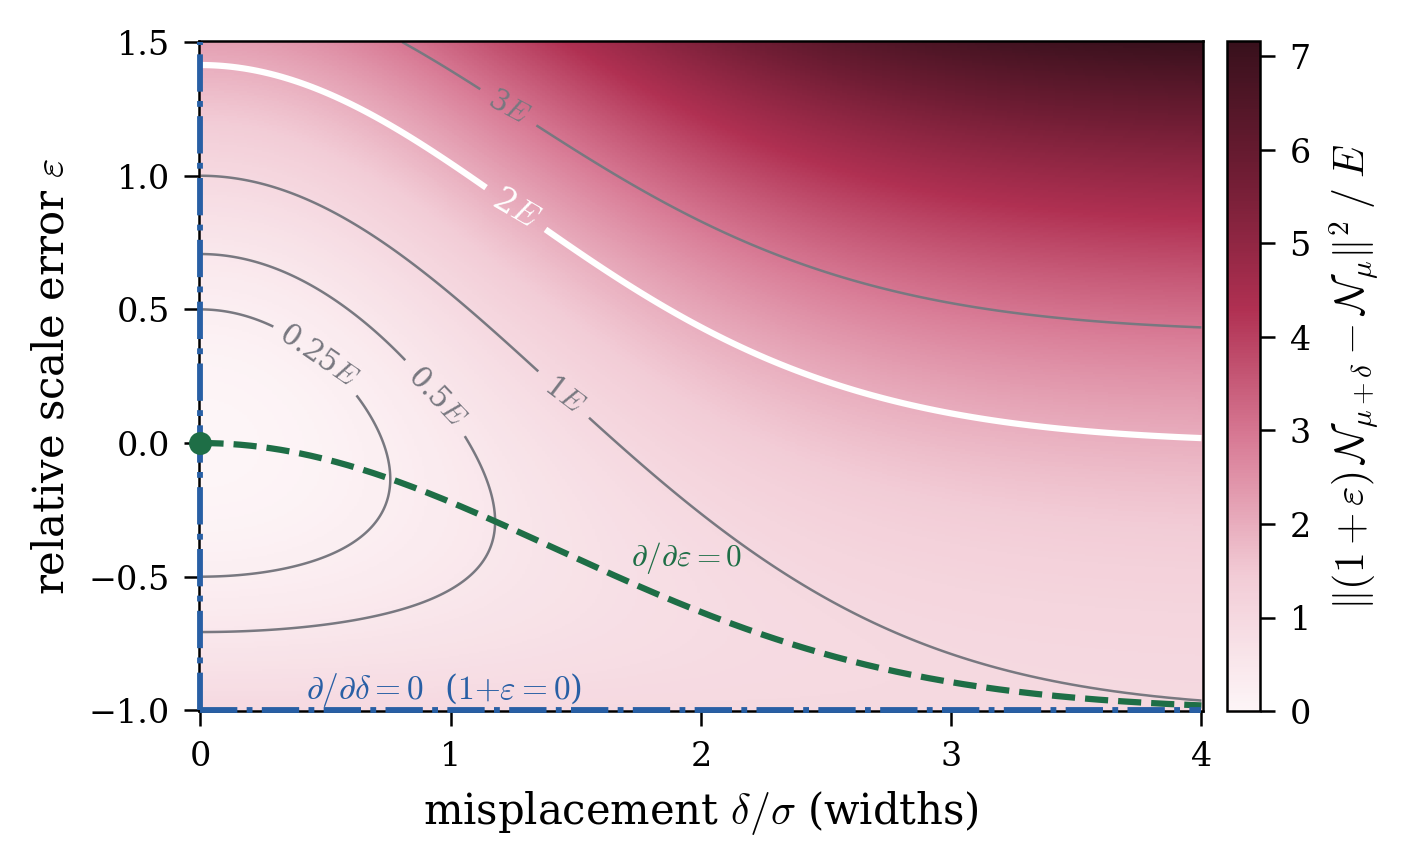
\includegraphics[width=\linewidth]{../figures/error_landscape/joint_error_heatmap.png}\\[2pt]
      {\scriptsize\color{soft} the joint landscape: the critical curves meet
      only at the truth --- the surface's one minimum.\par}
    \end{column}
  \end{columns}
\end{frame}

% ---------------------------------------------------------------- 25e-c Math: convergence and the training pull
\begin{frame}{The bowl and the training pull}
  \setlength{\abovedisplayskip}{3pt}
  \setlength{\belowdisplayskip}{3pt}
  \small
  Zoom into small $\delta$, $\varepsilon$ --- the regime of a converging
  network:
  \begin{columns}[T]
    \begin{column}{0.5\textwidth}
      \centering
      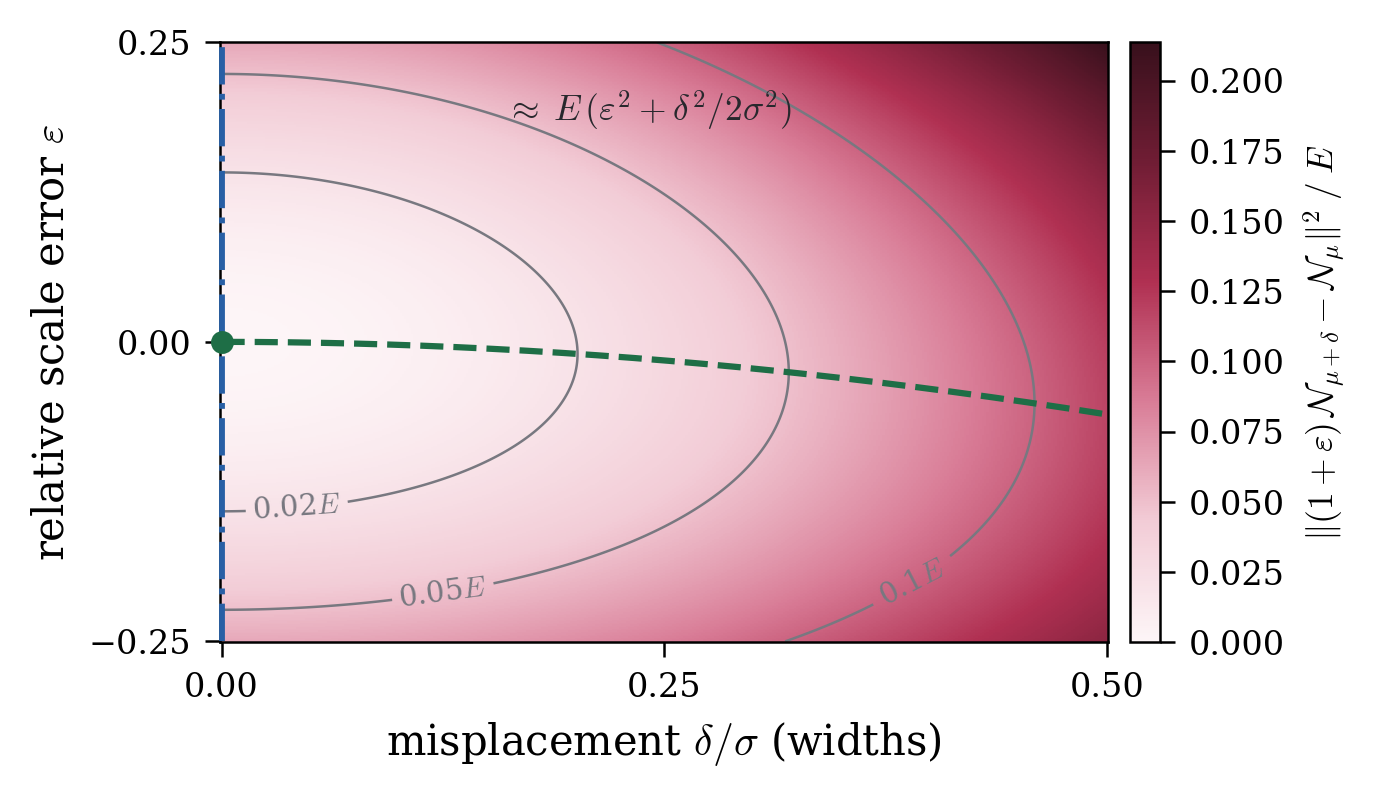
\includegraphics[width=\linewidth]{../figures/error_landscape/joint_error_convergence.png}
    \end{column}
    \begin{column}{0.5\textwidth}
      \centering
      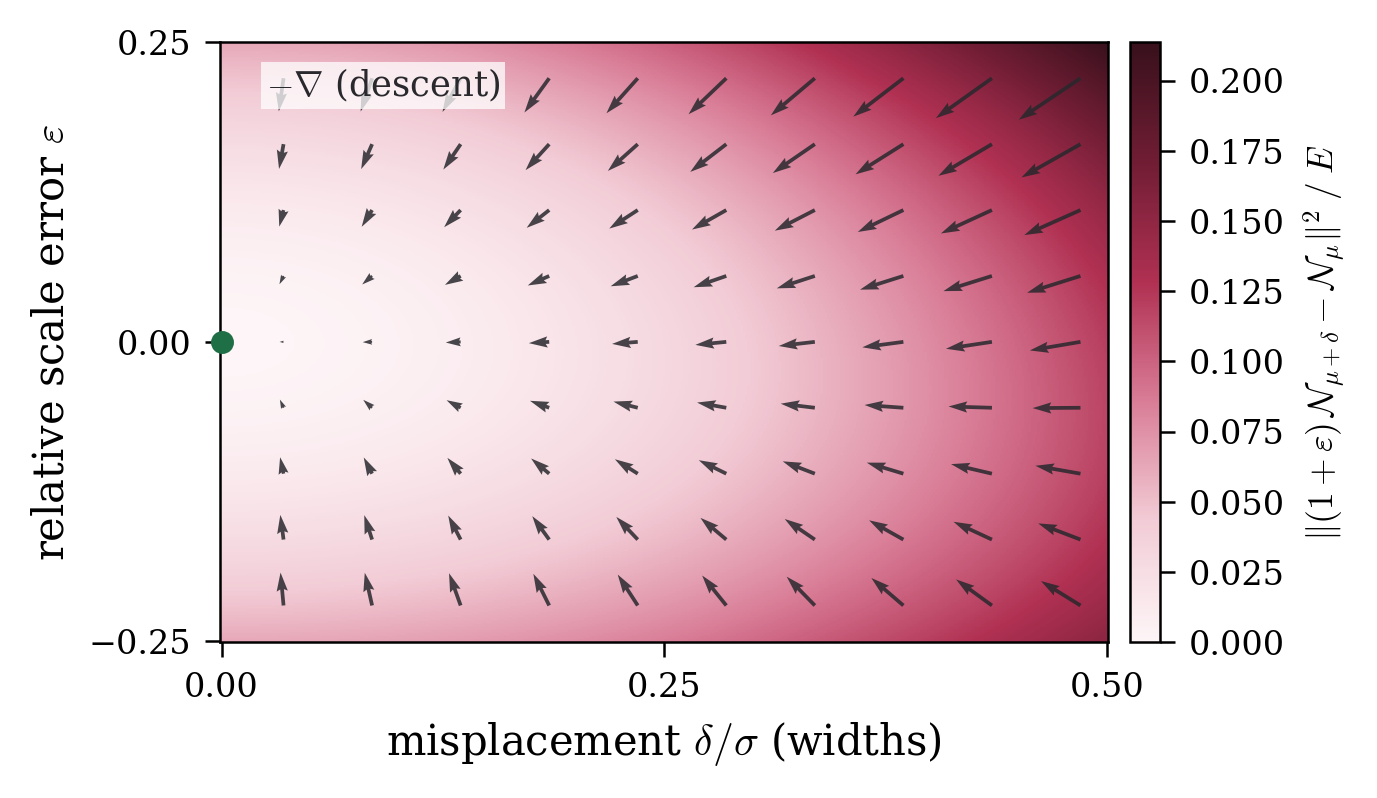
\includegraphics[width=\linewidth]{../figures/error_landscape/joint_error_gradient.png}
    \end{column}
  \end{columns}
  \smallskip
  {\scriptsize\color{soft} left: the quadratic bowl --- elliptic contours,
  valley tangent to $\varepsilon{=}0$, no plateau. right: the $-\nabla$
  descent field --- onto the valley at curvature $2E$, along it at $E$; its
  dim drift feeds the recall paradox (two frames ahead).\par}
\end{frame}

% ---------------------------------------------------------------- 25e-d Math: the K-scatterer sum decouples
\begin{frame}{The full profile --- separated scatterers decouple}
  \setlength{\abovedisplayskip}{3pt}
  \setlength{\belowdisplayskip}{3pt}
  \begin{columns}[c]
    \begin{column}{0.49\textwidth}
      \small
      \begin{itemize}
        \item \textbf{Write the error as residuals.} Truth and
              prediction are sums of $K$ components; Hungarian pairing matches
              them one to one, so pair $k$ owns its shift $\delta_k$ and scale
              error $\varepsilon_k$:
      \end{itemize}
      \[
      \begin{aligned}
        & p = \textstyle\sum_{k} \mathcal N_{\mu_k}, \qquad \hat p = \textstyle\sum_{k} (1{+}\varepsilon_k)\,\mathcal N_{\mu_k+\delta_k}\\[3pt]
        \Longrightarrow\;\; & \hat p - p \;=\; \textstyle\sum_{k} r_k, \qquad r_k = (1{+}\varepsilon_k)\,\mathcal N_{\mu_k+\delta_k} - \mathcal N_{\mu_k}
      \end{aligned}
      \]
      {\scriptsize\color{soft} $\mathcal N_{\mu_k}$: the $k$-th component
      $a_k\,\mathcal N(z;\mu_k,\sigma_k)$, energy
      $E_k=\lVert\mathcal N_{\mu_k}\rVert^2=a_k^2/(2\sqrt{\pi}\,\sigma_k)$;
      $r_k$: its residual.\par}
      \vspace{16pt}
      \begin{itemize}
        \item \textbf{Square the sum} --- bilinearity, no approximation:
      \end{itemize}
      \[
      \begin{aligned}
        & \lVert \hat p - p \rVert^2 \;=\; \textstyle\sum_{k} \lVert r_k \rVert^2 \;+\; 2\textstyle\sum_{j<k} \langle r_j, r_k \rangle\\[3pt]
        & \lVert r_k \rVert^2 \;=\; E_k\big[(1{+}\varepsilon_k)^2 + 1 - 2\,(1{+}\varepsilon_k)\,e^{-\delta_k^2/4\sigma_k^2}\big]
      \end{aligned}
      \]
    \end{column}
    \begin{column}{0.49\textwidth}
      \small
      \begin{itemize}
        \item \textbf{Assume the scatterers are separated.} Any two
              Gaussian components overlap in closed form --- exponentially
              small in the distance between their centres $m$, $m'$:
      \end{itemize}
      \[
      \begin{aligned}
        & \big\langle a_j\,\mathcal N(z;m,\sigma_j),\, a_k\,\mathcal N(z;m',\sigma_k) \big\rangle \\[2pt]
        & \;\propto\; e^{-(m-m')^2/2(\sigma_j^2+\sigma_k^2)}
      \end{aligned}
      \]
      \smallskip
      $\langle r_j, r_k\rangle$ is four such overlaps, centred near $\mu_j$
      and $\mu_k$. Assume the separation is big enough --- a few joint
      widths --- and all four cancel:
      \[
      \begin{aligned}
        & |\mu_j - \mu_k| \;\ge\; 3\,\sqrt{\sigma_j^2+\sigma_k^2}\\[2pt]
        \Longrightarrow\;\; & e^{-(\mu_j-\mu_k)^2/2(\sigma_j^2+\sigma_k^2)} \;\le\; e^{-9/2} \;\approx\; 0.01\\[2pt]
        \Longrightarrow\;\; & \hleq{\langle r_j, r_k\rangle \approx 0 \;\;\Longrightarrow\;\; \lVert\hat p - p\rVert^2 \;\approx\; \textstyle\sum_k \lVert r_k \rVert^2}
      \end{aligned}
      \]
    \end{column}
  \end{columns}
\end{frame}

% ---------------------------------------------------------------- 25f Math: the recall paradox
\begin{frame}{The recall paradox --- MSE turns doubt into dimming}
  \setlength{\abovedisplayskip}{4pt}
  \setlength{\belowdisplayskip}{4pt}
  \begin{columns}[c]
    \begin{column}{0.49\textwidth}
      \small
      \begin{itemize}
        \item \textbf{Squared error is minimised by the conditional mean} ---
              the value the loss pulls every output toward:
      \end{itemize}
      \[
        \hat a_2(x) \;=\; \mathrm E\,[\,a_2 \mid x\,]
      \]
      {\scriptsize\color{soft} $x$: the input patch; $a_2$: the second
      amplitude label --- defined as $0$ on pixels with a single scatterer
      ($K{=}1$).\par}
      \smallskip
      \begin{itemize}
        \item \textbf{Split the mean over the two cases.} The label is zero in
              one case and bright in the other; the zero case drops:
      \end{itemize}
      \[
      \begin{aligned}
        \hat a_2 \;&=\; \Pr(K{=}2\,|\,x)\,\mathrm E[a_2\,|\,K{=}2,x]\\[2pt]
        &\quad \;+\; \Pr(K{=}1\,|\,x)\,\mathrm E[a_2\,|\,K{=}1,x]\\[4pt]
        &\hleq{=\; \Pr(K{=}2\,|\,x) \cdot \mathrm E[a_2\,|\,K{=}2,x]}
      \end{aligned}
      \]
      \smallskip
      \begin{itemize}
        \item \textbf{Bayes' rule}, with $\pi=\Pr(K{=}2)$, and total
              probability over the two cases:
      \end{itemize}
      \[
      \begin{aligned}
        \Pr(K{=}2\,|\,x) \;&=\; \tfrac{p(x\,|\,K{=}2)\,\pi}{p(x\,|\,K{=}2)\,\pi \,+\, p(x\,|\,K{=}1)\,(1{-}\pi)}\\[3pt]
        &=\; \tfrac{\pi\,\Lambda}{1-\pi+\pi\,\Lambda}, \qquad
        \Lambda(x) \;=\; \tfrac{p(x\,|\,K{=}2)}{p(x\,|\,K{=}1)}
      \end{aligned}
      \]
\end{column}
    \begin{column}{0.49\textwidth}
      \small
      \begin{itemize}
        \item \textbf{$|A|$ runs:}
      \end{itemize}
      \[
      \begin{aligned}
        & \Lambda(x)\approx1\ \text{on every pixel} \ \Rightarrow\ \Pr(K{=}2\,|\,x)\approx\pi\\[1pt]
        & \Rightarrow\ \hat a_2 \ \text{pulled to} \ \pi\cdot\mathrm E[a_2\,|\,K{=}2,x]\\[2pt]
        & \Rightarrow\ \mathrm E[a_2\,|\,K{=}2,x] \;=\; f_\theta(P(x))\\[2pt]
        & \hleq{\hat a_2 \;=\; \pi\cdot f_\theta(P(x)) \ \text{--- dimmed}}\\[2pt]
        & \Rightarrow\ f_\theta(P(x)) \to 0, \ \text{class imbalance}
      \end{aligned}
      \]
      \smallskip
      \begin{itemize}
        \item \textbf{$\varphi$-only:} every pixel lands at an extreme:
      \end{itemize}
      \[
      \begin{aligned}
        & \Lambda(x)\gg1\ \text{on true pairs} \ \Rightarrow\ \Pr(K{=}2\,|\,x)\to1\\[1pt]
        & \hleq{\Rightarrow\ \hat a_2\to\mathrm E[a_2\,|\,K{=}2,x] \ \text{--- undimmed}}\\[2pt]
        & \hat a_2 = \mathrm E[a_2|K{=}2,x] = \mathrm E[a_2|K{=}2] = \bar a_2^{\mathrm{active}}\\[6pt]
        & \Lambda(x)\ll1\ \text{on singles} \ \Rightarrow\ \Pr(K{=}2\,|\,x)\to0\\[1pt]
        & \Rightarrow\ \hat a_2\to0 \ \text{--- the slot closes}
      \end{aligned}
      \]
    \end{column}
  \end{columns}
\end{frame}
